\documentclass[11pt,final,oneside]{fithesis}
\usepackage[utf8]{inputenc}
\usepackage[T1]{fontenc}
\usepackage{tipa}
\usepackage[slovak]{babel}
\usepackage{tabularx}
\usepackage{graphicx}
\usepackage{cite}
\usepackage{url}

\hbadness=1000
\tolerance=1000

\newcommand{\smalltt}[1]{\small\texttt{#1}\normalsize}

\thesistitle{Monitorování zátěže a využití výpočetních zdrojů v heterogenním výpočetním prostředí}
\thesissubtitle{Diplomová práca}
\thesisstudent{Juraj Leždík}
\thesiswoman{false}
\thesisfaculty{fi}
\thesisyear{jar 2016}
\thesisadvisor{Mgr. Miroslav Ruda}
\thesislang{sk}
\begin{document}

\FrontMatter
\ThesisTitlePage

\begin{ThesisDeclaration}
\DeclarationText
\AdvisorName
\end{ThesisDeclaration}


\begin{ThesisThanks}
\end{ThesisThanks}

\begin{ThesisAbstract}
\end{ThesisAbstract}

\begin{ThesisKeyWords}
\end{ThesisKeyWords}

\tableofcontents
\addcontentsline{toc}{chapter}{Obsah}

\MainMatter
\chapter{Úvod}

\chapter{Zber a uchovávanie časových rád}
\section{Časové rady}
Časová rada je sekvencia dát, kde danému časovému okamihu zodpovedá jedna hodnota. Príkladom je zaznamenávanie teplôt v priebehu roka, výšky oceánskeho prílivu alebo množstvo áut, ktoré za určitú dobu
prejde jedným bodom diaľnice. Efektívnou metódou vizuálizácie dát časových rád sú čiarové grafy. Horizontálna os reprezentuje plynutie času a na vertikálnej osi sú znázornené hodnoty v danom čase.

\subsection{Analýza časových rád}
Analýza časových rád sa primárne zaoberá získavaniu štatistík o zozbieraných dátach, napr. priemerná teplota počas celého roka. Medzi ďaľšie úlohy patrí:
\begin{description}
\item[\emph{Exploračná analýza dát}]
\item[\emph{Aproximácia na funkciu}] 
\item[\emph{Predpovedanie}] 
\item[\emph{Klasifikácia}] 
\end{description}
Mám sa viac o nich rozpísať?

\section{OpenTSDB}
OpenTSDB je databáza na uchovávanie a sprístupňovanie veľkých objemov časových dát. Pozostáva z Time Series Daemon (TSD) a z utilít pre príkazový riadok. Interakcia s OpenTSDB je primárne realizovaná cez jedného alebo viacerých TSD. Každý TSD je nezávislý.
Neexistuje žiadny riadiaci proces, žiadny zdieľaný stav, takže je možné spustiť toľko TSD, koľko je potrebné na zvládnutie požadovanej záťaže. Každý TSD používa open-source databázu HBase
na ukladanie a vyberanie dát časových rád. HBase schéma je vysoko optimalizovaná na rýchlu agregáciu podobných časových rád, aby minimalizovala požiadavky na úložný priestor. 
Používatelia TSD nemusia pristupovať do HBase priamo. S TSD je možné komunikovať cez jednoduchý protokol podobný Telnetu, cez HTTP API alebo cez jednoduché GUI. Všetka komunikácia
sa deje na tom istom porte (TSD odhadne protokol klienta pohľadom na prvých niekoľko bajtov, ktoré obdrží).\cite{openTSDB}

Na vizualizáciu dát existuje nástroj Metrilyx. Je to open-source webový engine, ktorý vytvára grafy zo zhromaždených dát. Je možné meniť časové rozpätie, za ktoré sa majú grafy metrík zobraziť .
\begin{figure}[h]
\begin{center}
       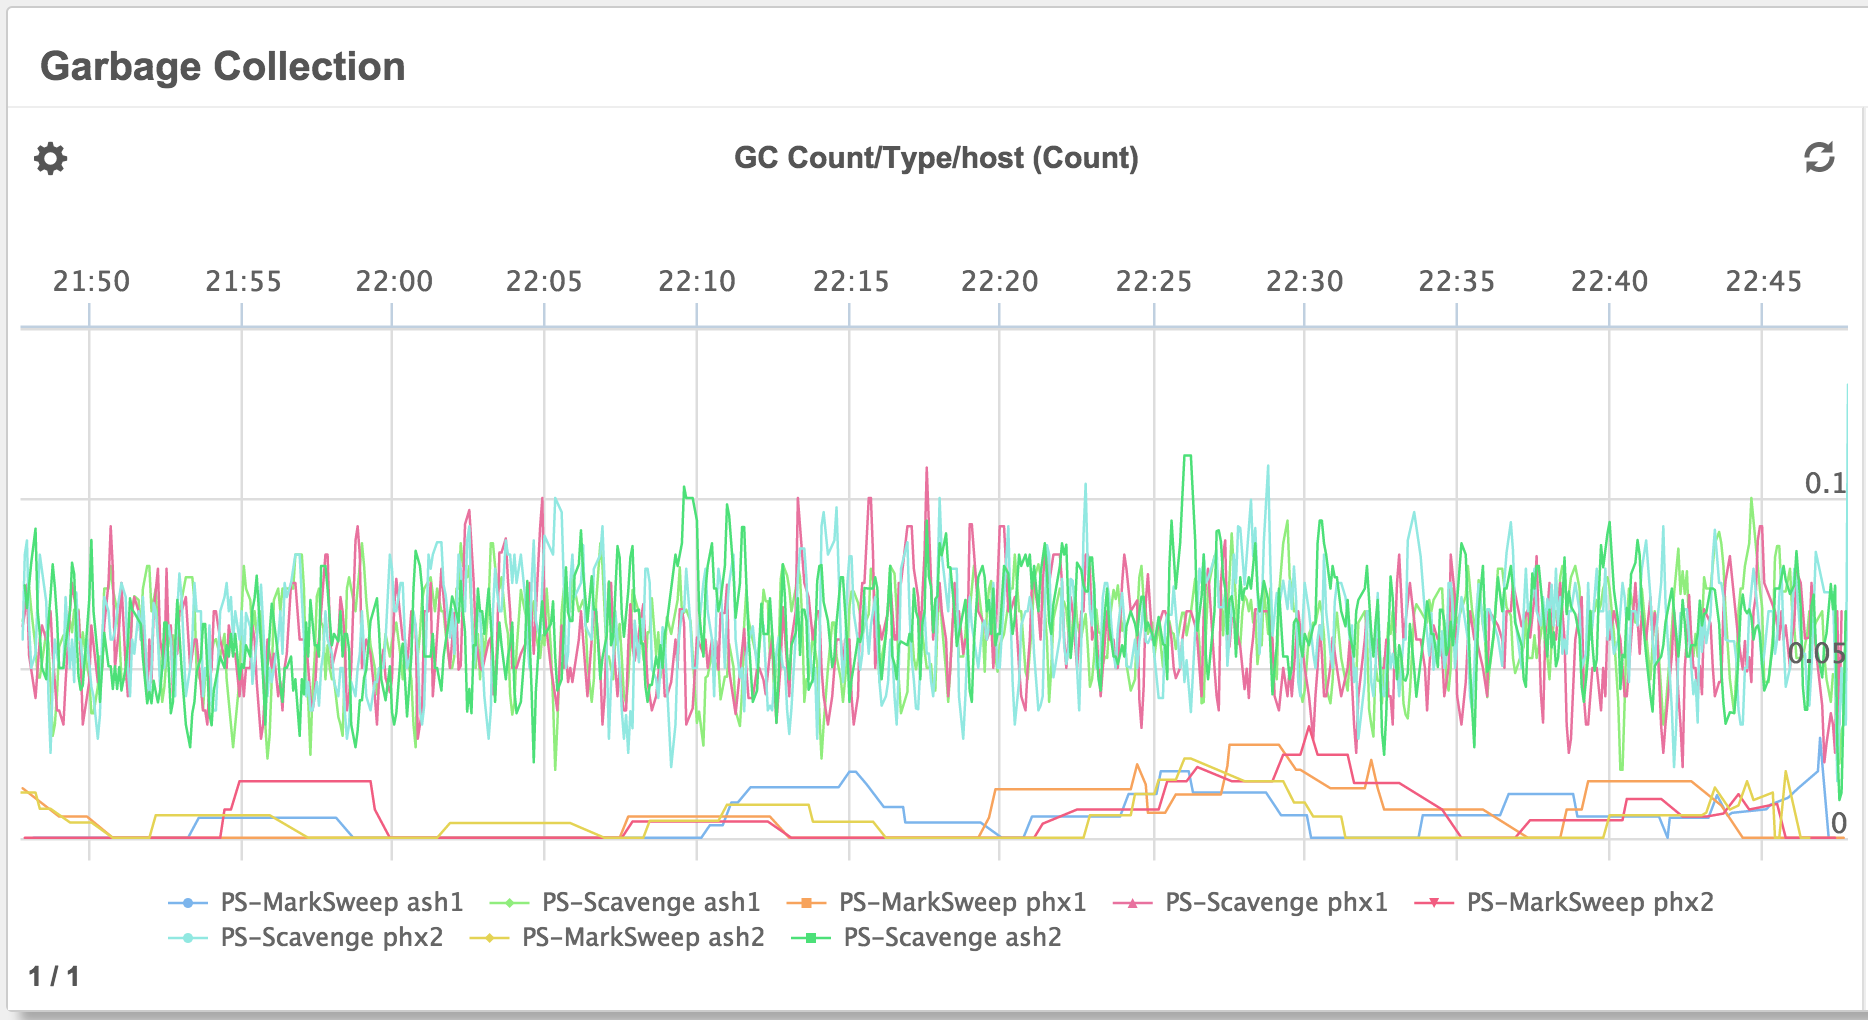
\includegraphics[width=0.8\textwidth]{images/metrilyx.png}
       \caption{Vizualizácia časových rád OpenTSDB pomocou Metrilyx}\cite{Metrilyx}
\end{center}
\end{figure}

\section{InfluxDB}
InfluxDB je platforma na zbieranie, uchovávanie, vizualizáciu a správu časových dát. Užívateľ môže vytvoriť viacero databáz. Dáta sa zapisujú a čítajú pomocou rozhrania príkazového riadka, 
rôznych klientskych knižníc, alebo pomocou HTTP API. Na vizualizáciu dát používa modul \emph{chronograf}.

\subsection{Politiky udržiavania}
Každá databáza obsahuje pravidlá, ktoré definujú, po akú dobu majú byť ukladané dáta časových rád a koľko kópií dát má byť vytvorených. Jedna databáza môže mať niekoľko takýchto politík. Pri zápise 
do nej je môžné špeicifikovať, ktorá politika sa má pre zápis použiť. Pri vytvorení databázy je automaticky vytvorená jedna politika

\subsection{Kontinuálne dotazovanie}
Databáza je schopná periodicky vykonávať požiadavky na dáta. Cieľom je zmenšovanie objemu dát. Ide o zhlukovanie dát s vysokou frekvenciou zberu, čím vzniknú dáta s menšou hustotou zberu. Táto hodnota je 
potom zvyčajne uložená do inej databázy.

\section{RRDTool}
RRDTool je nástroj na uchovávanie, spravovanie a vizuálizáciu časových dát. Využíva round-robin databázu. Je to databáza s dopredu danou maximálnou veľkosťou. V prípade, že príde požiadavka na zápis hodnoty 
a databáza je už plná, dôjde k prepisu nasjtaršej hodnoty. Tento nástroj takisto obsahuje funkcie na konsolidáciu dát. Konsolidovaná hodnota je typicky priemer, minimum alebo maximum z viacerých hodnôt zozbieraných 
za dlhší časový úsek. Tieto hodnoty sú ukladané do round-robin archívu.

\chapter{Aktuálne monitorovacie riešenia}
\section{Open-source}
\subsection{Nagios}
\subsubsection{PluginAPI}
Scripts and executables must do two things (at a minimum) in order to function as Nagios plugins:

Exit with one of several possible return values
Return at least one line of text output to STDOUT
The inner workings of your plugin are unimportant to Nagios. Your plugin could check the status of a TCP port, run a database query, check disk free space, or do whatever else it needs to check something. The details will depend on what needs to be checked - that's up to you.

Return Code

Nagios determines the status of a host or service by evaluating the return code from plugins. The following tables shows a list of valid return codes, along with their corresponding service or host states.

Plugin Return Code	Service State	Host State
\\0	OK	UP
\\1	WARNING	UP or DOWN/UNREACHABLE*
\\2	CRITICAL	DOWN/UNREACHABLE
\\3	UNKNOWN	DOWN/UNREACHABLE
\\Note Note: If the use_aggressive_host_checking option is enabled, return codes of 1 will result in a host state of DOWN or UNREACHABLE. Otherwise return codes of 1 will result in a host state of UP. The process by which Nagios determines whether or not a host is DOWN or UNREACHABLE is discussed here.

Plugin Output Spec

At a minimum, plugins should return at least one of text output. Beginning with Nagios 3, plugins can optionally return multiple lines of output. Plugins may also return optional performance data that can be processed by external applications. The basic format for plugin output is shown below:

TEXT OUTPUT | OPTIONAL PERFDATA
LONG TEXT LINE 1
LONG TEXT LINE 2
...
LONG TEXT LINE N | PERFDATA LINE 2
PERFDATA LINE 3
...
PERFDATA LINE N

The performance data (shown in orange) is optional. If a plugin returns performance data in its output, it must separate the performance data from the other text output using a pipe (|) symbol. Additional lines of long text output (shown in blue) are also optional.
\cite{01}

\subsubsection{Timeouty}

Format:	service_check_timeout=<seconds>
Example:	service_check_timeout=60
This is the maximum number of seconds that Nagios will allow service checks to run. If checks exceed this limit, they are killed and a CRITICAL state is returned. A timeout error will also be logged.

There is often widespread confusion as to what this option really does. It is meant to be used as a last ditch mechanism to kill off plugins which are misbehaving and not exiting in a timely manner. It should be set to something high (like 60 seconds or more), so that each service check normally finishes executing within this time limit. If a service check runs longer than this limit, Nagios will kill it off thinking it is a runaway processes.
\cite{02}


Nie je mechanizmus pre reštart alebo individuálne timeouty.
Má zastaralý Hadoop plugin, používa staré REST API.
Last Release Date 2010-11-05
\cite{03}

\subsection{Zabbix}
\subsubsection{Timeouty}
Timeout processing
Zabbix will not process a simple check longer than Timeout seconds defined in Zabbix server configuration file.
\cite{04}

Zabbix Agent
Timeout	 no	 1-30	3	Spend no more than Timeout seconds on processing
\cite{20}

Zabbix Server
Timeout	 no	 1-30	3	Specifies how long we wait for agent, SNMP device or external check (in seconds).
\cite{05}

Neuvádza sa nič o zastavovaní procesov.
\subsubsection{Moduly}

Loadable modules offer a performance-minded option for extending Zabbix functionality.

There already are ways of extending Zabbix functionality by way of:

user parameters (agent metrics)
external checks (agent-less monitoring)
system.run[] Zabbix agent item.
They work very well, but have one major drawback, namely fork(). Zabbix has to fork a new process every time it handles a user metric, which is not good for performance. It is not a big deal normally, however it could be a serious issue when monitoring embedded systems, having a large number of monitored parameters or heavy scripts with complex logic or long startup time.

Zabbix 2.2 comes with support of loadable modules for extending Zabbix agent, server and proxy without sacrificing performance.

A loadable module is basically a shared library used by Zabbix daemon and loaded on startup. The library should contain certain functions, so that a Zabbix process may detect that the file is indeed a module it can load and work with.

Loadable modules have a number of benefits. Great performance and ability to implement any logic are very important, but perhaps the most important advantage is the ability to develop, use and share Zabbix modules. It contributes to trouble-free maintenance and helps to deliver new functionality easier and independently of the Zabbix core code base.
\cite{06}

\subsection{Icinga}
By default the Icinga 2 daemon is running as icinga user and group using the init script. Using Debian packages the user and group are set to nagios for historical reasons.
\cite{07}

\subsubsection{Externé pluginy}
Icinga determines the status of a host or service by evaluating the return code from plugins. The following tables shows a list of valid return codes, along with their corresponding service or host states
\cite{08}

\subsubsection{Notifikácie a príkazy udalostí}
Unlike notifications, event commands for hosts/services are called on every check execution if one of these conditions match:
The host/service is in a soft state
The host/service state changes into a hard state
The host/service state recovers from a soft or hard state to OK/Up

Ide len o spustenie nejakého systémového príkazu.
\cite{09}

\subsubsection{Itegrácie s aplikáciami} 
these tiny pure shell+awk plugins for monitoring your hadoop cluster are a enhanced and uptodate version of exchange.nagios.org check_hadoop-dfs.sh
\cite{10}

\subsection{Cacti}
Cacti is a complete network graphing solution designed to harness the power of RRDTool's data storage and graphing functionality. Cacti provides a fast poller, advanced graph templating, multiple data acquisition methods, and user management features out of the box.
\cite{11}

\subsection{collectd}
There are some key differences we think set collectd apart. For one, it's written in C for performance and portability, allowing it to run on systems without scripting language or cron daemon, such as embedded systems. 
At the same time it includes optimizations and features to handle hundreds of thousands of data sets. It comes with over 90 plugins. It provides powerful networking features and is extensible in numerous ways. 

\subsubsection{Obmedzenia}
It does not generate graphs. It can write to RRD files, but it cannot generate graphs from these files. 
Monitoring functionality has been added in version 4.3, but is so far limited to simple threshold checking. 
\cite{12}

\subsubsection{Zapisovací plugin Write TSDB}
The Write TSDB plugin writes metrics to OpenTSDB, an open-source distributed time-series database based on Apache HBase.
\cite{13}

\begin{description}
\item[\emph{Host Address}] Hostname or address to connect to. Defaults to localhost.
\item[\emph{Port Service}] Service name or port number to connect to. Defaults to 4242.
\item[\emph{HostTags String}] When set, HostTags is added to the end of the metric. It is intended to be used for name=value pairs that the TSD will tag the metric with. Dots and whitespace are not escaped in this string.
\item[\emph{StoreRates false|true}] If set to true, convert counter values to rates. If set to false (the default) counter values are stored as is, as an increasing integer number.
\item[\emph{AlwaysAppendDS false|true}] If set the true, append the name of the Data Source (DS) to the "metric" identifier. If set to false (the default), this is only done when there is more than one DS.
\end{description}

\subsubsection{Prahy a notifikácie}

The only action the Threshold plugin takes itself is to generate and dispatch a notification. Every time a value is out of range, 
notification is dispatched. 
Also, all values that match a threshold are considered to be relevant or "interesting". As a consequence collectd will issue a notification 
if they are not received for Timeout iterations.  for example, Timeout is set to "2" (the default) and some hosts sends it's CPU statistics to the server every 60 seconds, a notification will be dispatched after about 120 seconds. It may take a little longer because the timeout is checked only once each Interval on the server.

When a value comes within range again or is received after it was missing, an "OKAY-notification" is dispatched.
\cite{14}

\subsection{Ostatne} 
\begin{description}
\item[\emph{Zenoss}]
\item[\emph{Munin}]
\end{description}

\section{Ganglia} 
Ganglia is a scalable distributed monitoring system for high-performance computing systems such as clusters and Grids. It is based on a hierarchical design targeted at federations of clusters. It leverages widely used technologies such as XML for data representation, XDR for compact, portable data transport, and RRDtool for data storage and visualization. It uses carefully engineered data structures and algorithms to achieve very low per-node overheads and high concurrency. The implementation is robust, has been ported to an extensive set of operating systems and processor architectures, and is currently in use on thousands of clusters around the world. It has been used to link clusters across university campuses and around the world and can scale to handle clusters with 2000 nodes.
Ganglia is a BSD-licensed open-source project that grew out of the University of California, Berkeley Millennium Project
\cite{15}
Pre Gangliu je dostupný monitorovací plugin pre Hadoop.
\cite{16}

\section{Komerčné riešenia}

\section{Torque}
Nenašiel som žiadne komerčný softvér na monitorovanie Torque. 

\section{libvirt/KVM}

\section{Docker}
\subsection{Scout}
Scout runs within Docker containers without any special configuration. \cite{scout}

\subsection{New Relic}
http://newrelic.com/docker

\subsection{AppDynamics}
https://www.appdynamics.com/community/exchange/extension/docker-monitoring-extension/


\section{Hadoop}
\subsection{New Relic}
http://newrelic.com/plugins

\subsection{AppDynamics}
The Hadoop monitoring extension captures metrics from Hadoop Resource Manager and/or Apache Ambari and displays them in Appdynamics Metric Browser.

This extension works only with the standalone machine agent.


Metrics include:

Hadoop Resource Manager
App status and progress: submitted, pending, running, completed, killed, and failed app count
Memory size, memory usage
Allocated containers, container count in different states
Node status, count of nodes in different states
Scheduler capacity, app and container count
Ambari
Individual host metrics including CPU, disk, memory, JVM, load, network, process, and RPC metrics
Service component metrics including CPU, disk, memory, JVM, load, network, process, RPC, and component-specific metrics
\cite{17}

\chapter{Cloudové technológie}

\section{Dávkové úlohy}
\subsection{Torque}
TORQUE Resource Manager poskytuje kontrolu nad dávkovými úlohami a distribuovanými výpočetnými zdrojmi. Je to pokročilý open-source product, založený na na pôvodnom PBS projekte. 
Zahŕňa vyznamné pokroky v oblastiach škálovania, spoľahlivosti a funkcionality a je v súčasnosti používaný desiatkami tisícov vládnych, akademických a komerčných webových stránok po celom svete. Torque môže byť voľne používaný, modifikovaný a distribuovaný je v rámci obmedzení svojou licenciou.\cite{torque}

Monitorovanie tejto aplikácie bude prebiehat prostredníctvom volania jej ovládacích príkazov:
\begin{description}
\item[\emph{momctl}] - sledovanie záťaže riadiaceho procesu a zisťovanie, ktoré úlohy sa práve spracovávajú
\item[\emph{printjob}] - sledovanie zdrojov, ktoré spotrebováva konkrétna úloha 
\end{description}



\section{Aplikačné kontajnery}
Kontajnery predstavujú odlišný prístup k virtualizácií ako virtuálne stroje. Tiež ide o snahu spúšťať softvér v prostredí oddelenom od skutočného hardvéru a operačného systému. Na rozdiel od úplných virtuálnych strojov 
nie je virtualizovaný celý hardvér, ale len softvérové vybavenie nevyhnutné na spustenie programu. Rozdiel v architektúre ilustruje nasledovný obrázok: 
\begin{figure}[h]
\begin{center}
       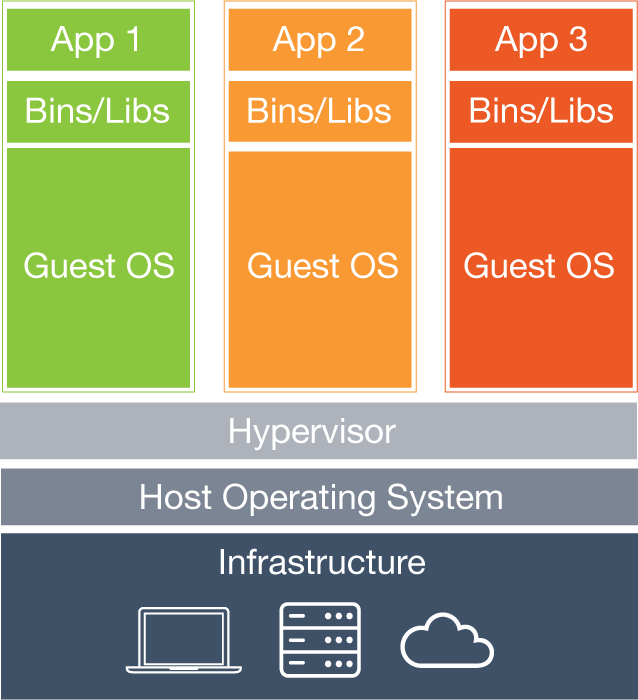
\includegraphics[width=0.8\textwidth]{images/docker.png}
       \caption{Porovnanie architektúry Docker a virtuálnych strojov}\cite{docker}
\end{center}
\end{figure}
V kontajneri môže byť spustený nezávislý operačný systém spolu s požadovanými aplikáciami. Hosťovský počítač, na ktorom sú kontajnery spustené, má jeden operačný systém a jednu množinu prostriedkov, 
ktoré tieto kontajnery zdieľajú. Jednotlivé kontajnery dostávajú kontrolovaný prístup k výpočtovému výkonu, pamäti, úložnej kapacite, sieti a prípadne ďalším prostriedkom.

\subsection{Linux cgroups}
Linux cgroups je technológia linuxového jadra, ktorá umožňuje limitovať, sledovať a izolovať spotrebu prostriedkov systému jednotlivými procesmi. Zavádza stromovo organizované kontrolné skupiny. 
Kontrolná skupina obsahuje obmedzenia pre jeden systémový prostriedok, tzv. susbsystém. Príklad subsystémov, ktoré poskytuje Red Hat Enterprise Linux: 
\begin{description}
\item[\emph{blkio}] - this subsystem sets limits on input/output access to and from block devices such as physical drives (disk, solid state, USB, etc.).
\item[\emph{cpu}] - this subsystem uses the scheduler to provide cgroup tasks access to the CPU.
\item[\emph{cpuacct}] - this subsystem generates automatic reports on CPU resources used by tasks in a cgroup.
\item[\emph{cpuset}] - this subsystem assigns individual CPUs (on a multicore system) and memory nodes to tasks in a cgroup.
\item[\emph{devices}] - his subsystem allows or denies access to devices by tasks in a cgroup.
\item[\emph{freezer}] - this subsystem suspends or resumes tasks in a cgroup.
\item[\emph{memory}] - this subsystem sets limits on memory use by tasks in a cgroup, and generates automatic reports on memory resources used by those tasks.
\item[\emph{net_cls}] - this subsystem tags network packets with a class identifier (classid) that allows the Linux traffic controller (tc) to identify packets originating from a particular cgroup task.
\item[\emph{net_prio}] - this subsystem provides a way to dynamically set the priority of network traffic per network interface.
\item[\emph{ns}] - the namespace subsystem.
\end{description}

Pre každý subsystém existuje jeden strom kontrolných skupín. Ďalej skupina obsahuje zoznam procesov, ktoré podliehajú definovaným obmedzeniam. V strome kontrolných skupín sa proces vyskystuje len raz.


\subsection{Docker}
Docker umožňuje zabaliť aplikáciu so všetkými jej závislosťami do štandardizovanej jednotky (tzv. kontajnery) určenej na softvérový vývoj. Kontajnery Dockeru obaľujú softvér kompletným súborovým systémom, ktorý
zahŕňa všetko, čo daný softvér potrebuje na spustenie: kód, nástroje potrebné na beh, systémové nástroje a knižnice. Toto zaručuje, že program bude pracovať rovnako bez ohľadu na prostredie, v ktorom
je spustený.\cite{docker}


\section{Virtuálne stroje}
Virtuálne stroje poskytujú úplnú virtualizáciu. Na jednom hosťujúcom počítači môže byť spustených viacero virtuálnych strojov. Každý má svoj vlastný virtuálny procesor, pamäť, grafický procesor, pevný disk 
a periférie. Operačný systém spustený vo virtuálnom stroji je izolovaný od hosťovského opračného systému (ak ho hosťovský počítač má). Takéto riešenie má jednu bezpečnostnú výhodu oproti aplikačným 
kontajnerom. Nežiadúce fungovanie jedného virtuálneho stroja neovplyvňuje beh ostatných.
V súčasnosti existuje mnoho úrovní virtuálnych strojov. Emulácia inštrukčnej sady, prekladanie programov za beho a ich optimalizácia, vysokoúrovňové virtuálne stroje (napr. Java) a systémové virtuálne stroje používané ako
jednotlivcami tak na serveroch.

\subsection{Hypervízor}
Hypervízor je softvér, ktorý vytvára a zabezpečuje beh virtuálnych strojov. Rozlišujeme 2 typy:
\begin{description}
\item[natívny] - na hosťujúcom počítači nie je nainštalovaný žiadny operačný systém. Hypervízor spravuje hardvér hosťujúceho počítača a kontroluje beh operačných systémov, ktoré sa javia ako procesy.
Príkladom je VMware ESX/ESXi, Oracle VM Server for x86 alebo Citrix XenServer.
\item[hosťovaný] - hypervízor je spustený ako bežný program v operačnom systéme hosťujúceho počítača. Príkladom je QEMU, VMware Workstation alebo VirtualBox.
\end{description}
\cite{hypervisorTypes}

\subsection{libvirt/KVM}
KVM\footnotemark\footnotetext{Kernel-based Virtual Machine} je plné virtualizačné riešenie pre Linux pre x86 hardvér, obsahujúce virtualizačné rozšírenia (Intel VT or AMD-V).
Pozostáva z nahrateľného modulu jadra, kvm.ko, ktorý poskytuje základ virtualizačnej infraštruktúry a šepcifický modul, kvm-intel.ko alebo kvm-amd.ko. Je možné virtualizovať obrazy 
s operačným systémami Linux aj Windows. Každý virtuálny stroj má vlastný virtualizovaný hardvér: sieťovú kartu, disk, grafický adaptér, atď. KVM je open-source softvér. Virtualizačný modul jadra
sa nachádza v Linuxe od verzie 2.6.20.\cite{kvm}

libvirt je sada nástrojov na prácu s virtualizačnými schopnosťami Linuxu (a ostatných OS). Je to voľný softvér dostupný pod licenciou GNU LGPL. 
Obsahuje API v jazyku C a väzby pre bežné programovacie jazyky.\cite{libvirt}


\section{MapReduce aplikačné prostredia}
\subsection{Hadoop}
Projekt Apache Hadoop vyvíja open-source softvér na spoľahlivé, škálovateľné, distribuované výpočty. Apache Hadoop je prostredie, ktoré umožňuje distribuované spracovávanie veľkých množstiev dát
naprieč clustermi, používajúcimi jednoduché programovacie modely. Je navrhnutý tak, aby bol škálovateľný od jednotlivých serverov po tisícky strojov, kde každý poskytuje lokálny výpočetný výkon a úložný priestor.
Nespolieha sa na vysokú dosupnosť hardvérových prostriedkov, ale je navrhnutý, aby detekoval a zvládal chyby na aplikačnej vrstve, takže poskytuje vysoko dostupnú službu nad clusterom počítačov, z ktorých 
každý je náchylný na chyby.

Projekt pozostáva z týchto modulov:

\begin{description}
\item[\emph{Hadoop Common:}] spoločné nástroje, ktoré podporujú ostatné Hadoop moduly
\item[\emph{Hadoop Distributed File System (HDFS™):}] distribuovaný súborový systém, ktorý poskytuje vysokú priepustnosť
\item[\emph{Hadoop YARN:}] prostredie pre plánovanie úloh a správu zdrojov clustera
\item[\emph{Hadoop MapReduce:}] systém založený na YARN pre paralelné spracovávanie veľkých množstiev dát, prostredie pre plánovanie úloh a správu zdrojov clustera
\end{description}

\chapter{Metriky}
\section{Torque}
\subsection{Technika zbierania metrík}
Na zbieranie metrík som použil príkaz \emph{qstat -j}.

			Prints either for all pending jobs  or  the  jobs  con-
          tained  in  job_list  various information. The job_list
          can contain job_ids, job_names, or wildcard  expression
          sge_types(1).

          For  jobs  in  E(rror)  state  the  error   reason   is
          displayed. For jobs that could not be dispatched during
          in the  last  scheduling  interval  the  obstacles  are
          shown, if 'schedd_job_info' in sched_conf(5) is config-
          ured accordingly.

          For running  jobs  available  information  on  resource
          utilization   is  shown  about  consumed  cpu  time  in
          seconds,  integral  memory  usage  in  Gbytes  seconds,
          amount  of  data  transferred in io operations, current
          virtual memory utilization in Mbytes, and maximum  vir-
          tual  memory utilization in Mbytes. This information is
          not available if resource utilization retrieval is  not
          supported for the OS platform where the job is hosted.
          
\subsection{Zbierané metriky}
Príkaz qstat -j poskytuje viacero režimov výstupu.
\begin{description}
\item[\emph{Cluster Queue Format}]
\\
\begin{enumerate}
\item[] the cluster queue name
\item[] an average of the normalized load average  of  all  queue
        hosts.
\item[] the number of currently used slots.
\item[] the number of slots reserved in advance.
\item[] the number of currently available slots.
\item[] the total number of slots.
\item[] the number of slots which is  in  at  least  one  of  the states  'aoACDS' and in none of the states 'cdsuE'
\item[] the number of slots which are in one of these  states  or in any  combination of them: 'cdsuE'
\end{enumerate}

\item[\emph{Reduced Format}]
\\
\begin{enumerate}
\item[]the job ID.
\item[]the priority of the job determining its position  in  the
        pending  jobs  list.
\item[] the name of the job,
\item[] the user name of the job owner.
\item[] the status of the  job  -  one  of  d(eletion),  E(rror),
        h(old), r(unning), R(estarted), s(uspended), S(uspended),
        t(ransfering), T(hreshold) or w(aiting).
\item[] the submission or start time and date of the job.
\item[] the  queue  the  job  is  assigned  to  (for  running  or
        suspended jobs only).
\item[] the number of job slots or the function of  parallel  job
        tasks if -g t is specified.
\item[] the array job task id. Will be empty for non-array  jobs.
        See  the  -t option to qsub(1) and the -g above for addi-
        tional information.
\end{enumerate}
     If the -t option is supplied, each status line  always  con-
     tains  parallel  job task information as if -g t were speci-
     fied and each line contains the following parallel job  sub-
     task information:
\begin{enumerate}
\item[] the parallel task ID (do not confuse parallel tasks  with
        array job tasks),
\item[] the status of the  parallel  task  -  one  of  r(unning),
        R(estarted),   s(uspended),   S(uspended),   T(hreshold),
        w(aiting), h(old), or x(exited).
\item[] the cpu, memory, and I/O usage,
\item[] the exit status of the parallel task,
\item[] and the failure code and message for the parallel task.
\end{enumerate}

\item[\emph{Full Format}]
\\
\begin{enumerate}
\item[] the queue name
\item[] the  queue  type  -  one   of   B(atch),   I(nteractive),
        C(heckpointing),  P(arallel),  T(ransfer) or combinations
        thereof or N(one),
\item[] the number of used and available job slots
\item[] the load average of the queue host,
\item[] the architecture of the queue host and
\item[] the state  of  the  queue  -  one  of  u(nknown)  if  the
        corresponding  sge_execd(8) cannot be contacted, a(larm),
        A(larm),     C(alendar      suspended),      s(uspended),
        S(ubordinate),  d(isabled), D(isabled), E(rror) or combi-
        nations thereof.
\item[] resource availability information
     is  printed  following  the  queue  status  line.  
\item[] the job ID,
\item[] the priority of the job determining its position  in  the
        pending  jobs  list. 
\item[] the job name,
\item[] the job owner name,
\item[] the status of the job - one of t(ransfering),  r(unning),
        R(estarted), s(uspended), S(uspended) or T(hreshold) (see
        the Reduced Format section for detailed information),
\item[] the submission or start time and date of the job.
\item[] the number of job slots or the function of  parallel  job
        tasks if -g t is specified.
\end{enumerate}

If the -t option is supplied, each job status line also con-
     tains
     \begin{enumerate}

\item[] the task ID,
\item[] the status of the task - one of  r(unning),  R(estarted),
        s(uspended), S(uspended), T(hreshold), w(aiting), h(old),
        or x(exited) (see the Reduced Format section for detailed
        information),
\item[] the cpu, memory, and I/O usage,
\item[] the exit status of the task,
\item[] and the failure code and message for the task.
\end{enumerate}
\end{description}
 
Potrebné metriky poskytuje prepínač -t v redukovanom formáte, preto som použil túto metódu výstupu.

\section{Docker}
Buem zberať metriky o spotrebovávaných zdrojoch pre každý kontajner.

\subsection{Technika zbierania metrík}
Na komunikáciu s Dockerom je možné využiť:
\begin{description}
\item[príkazy aplikácie v príkazovom riadku]
\item[Remote API]
\end{description}

Používanie príkazov aplikácie môže byť o čosi rýchlejšie, ale následne by bolo potrebné analyzovať textový výstup programu.
Rozhodol som sa použiť Remote API. Toto API funguje pre účely monitorovania na princípe REST a odpovede vracia vo formáte JSON, čo predstavuje zjednodušenie spracovania výstupu. Démon Dockeru "počúva" na 
lokálnom sockete, čo by nemalo spôsobovať výrazné oneskorenie odpovede.

O každom kontajneri spustenom v Dockeri budem sledovať využívanie týchto zdrojov :
\begin{description}
\item[\emph{procesor}]
\item[\emph{pevný disk}]
\item[\emph{sieť}]
\item[\emph{pamäť}]
\end{description}

  
Dáta je možné zberať buď ako prúd, alebo po jednorazových žiadostiach. To ešte nemám veľmi preštudované, neviem aké sú tam intervaly, tak sa rozhodnem až neskôr.
Predpokladám ale, že z hľadiska rýchlosti a alokácie bude cesta asi ten stream.

\subsection{Sieť}
Aby mohli medzi sebou jednotlivé kontajnery komunikovať, Docker im poskytuje sieťové rozhrania. Každé rozhranie má nakonfigurovanú sieť,
do ktorje patrí. Na to, aby kontajnery spolu mohli komunikovať, musia byť členmi rovnakej siete. Komunikácia naprieč sieťami nie je možná.
Užívatelia si môžu definovať vlastné siete. Docker na vytvorenie týchto sietí poskytuje dva ovládače.

\subsubsection{Sieť typu most}
Je to jednoduchý typ siete určený pre malé siete. Je ju možné vytvoriť príkazom 
\\
{\em \$ docker network create --driver bridge NÁZOV\_SIETE}
\\ \\
Po vytvorení siete je možné spustiť kontajnery v tejto sieti príkazom
\\ \\
{\em \$ docker run --net=NÁZOV\_SIETE --name=NÁZOV\_KONTAJNERA}

\subsubsection{Prekladaná sieť}
Docker umožňuje vytvoriť aj sieť, v ktorej sa nachádza viacero hostov zároveň. To umožňuje komunikovať medzi sebou aj kontajnerom,
ktoré sú spustené v rozličných k a ani na jednom hoste.
An overlay network

\subsubsection{Metriky siete}
Pre jednotlivé sieťové rozhrania je možné zbierať tieto metriky:
\begin{description}
\item[rx_bytes] - počet prijatých bajtov
\item[rx_dropped] - počet prichádzajúcich zahodených bajtov
\item[rx_error] - počet chybných bajtov
\item[rx_packets] - počet prijatých paketov
\item[tx_bytes] - počet odoslaných bajtov
\item[tx_dropped] - počet zahodených bajtov pri pokuse o odoslanie
\item[tx_errors] - počet odoslaných chybných bajtov
\item[tx_packets] - počet odoslaných paketov
\end{description}

\subsection{Pamäť}
\\
\begin{description}
\item[usage] - spotreba pamäte
\item[failcnt] - počet chýb
\end{description}

\subsection{Procesor}
\\        cpu_usage 
\\           percpu_usage
\\              16970827,
\\              1839451,
\\              7107380,
\\              10571290
\\           usage_in_usermode"
\\           total_usage" 
\\           usage_in_kernelmode" 
\\        system_cpu_usage

\section{libvirt/KVM}
\subsection{Technika zbierania metrík}
Na monitorovanie virtuálnych strojov použijem existujúcu implementáciu sond v jazyku Python. Je šírená pod licenciou open-source a vznika v rámci organizácie Cesnet. 

\subsection{Metriky siete}
Pre jednotlivé sieťové rozhrania je možné zbierať tieto metriky:
\begin{description}
\item[rx_bytes] - počet prijatých bajtov
\item[rx_dropped] - počet prichádzajúcich zahodených bajtov
\item[rx_error] - počet chybných bajtov
\item[rx_packets] - počet prijatých paketov
\item[tx_bytes] - počet odoslaných bajtov
\item[tx_dropped] - počet zahodených bajtov pri pokuse o odoslanie
\item[tx_errors] - počet odoslaných chybných bajtov
\item[tx_packets] - počet odoslaných paketov
\end{description}

\subsection{Metriky pamäte}
\begin{description}
\item[VIR_DOMAIN_MEMORY_STAT_SWAP_IN] - The total amount of memory written out to swap space (in kB).
\item[VIR_DOMAIN_MEMORY_STAT_SWAP_OUT] - Page faults occur when a process makes a valid access to virtual memory that is not available. When servicing the page fault, if disk IO is required, it is considered a major fault. If not, it is a minor fault. These are expressed as the number of faults that have occurred.
\item[VIR_DOMAIN_MEMORY_STAT_MAJOR_FAULT] - počet chybných bajtov
\item[VIR_DOMAIN_MEMORY_STAT_MINOR_FAULT] - počet prijatých paketov
\item[VIR_DOMAIN_MEMORY_STAT_UNUSED] - The amount of memory left completely unused by the system. Memory that is available but used for reclaimable caches should NOT be reported as free. This value is expressed in kB.
\item[VIR_DOMAIN_MEMORY_STAT_AVAILABLE] - The total amount of usable memory as seen by the domain. This value may be less than the amount of memory assigned to the domain if a balloon driver is in use or if the guest OS does not initialize all assigned pages. This value is expressed in kB.
\item[VIR_DOMAIN_MEMORY_STAT_ACTUAL_BALLOON] - Current balloon value (in KB).
\item[VIR_DOMAIN_MEMORY_STAT_RSS] - Resident Set Size of the process running the domain. This value is in kB
\item[VIR_DOMAIN_MEMORY_STAT_NR] - The number of statistics supported by this version of the interface. To add new statistics, add them to the enum and increase this value.
\end{description}

\subsection{Metriky zápisu dát}
\begin{description}
\item[rd_req] - number of read requests
\item[rd_bytes] - number of read bytes
\item[wr_req] - number of write requests
\item[wr_bytes] - number of written bytes
\item[errs] - In Xen this returns the mysterious 'oo_req'.
\end{description}

\subsection{Metriky CPU}
V dokumentácií sa presne neuvádza, budem musieť zstiť z implementácie.


\section{Hadoop}

\subsection{Technika zbierania metrík}
The Hadoop YARN web service REST APIs are a set of URI resources that give access to the cluster, nodes, applications, and application historical information. 
The URI resources are grouped into APIs based on the type of information returned. Some URI resources return collections while others return singletons.
HTTP Requests

To invoke a REST API, your application calls an HTTP operation on the URI associated with a resource.

Summary of HTTP operations

Currently only GET is supported. It retrieves information about the resource specified.

Security

The web service REST API’s go through the same security as the web UI. 

\cite{18}

\subsection{Dostupné metriky}
\subsubsection{Cluster Metrics API}
Toto API poskytuje metriky o celom clusteri.
\begin{description}
\item[appsSubmitted] - The number of applications submitted
\item[appsCompleted] - The number of applications completed
\item[appsPending] - The number of applications pending
\item[appsRunning] - The number of applications running
\item[appsFailed] - The number of applications failed
\item[appsKilled] - The number of applications killed
\item[reservedMB] - The amount of memory reserved in MB
\item[availableMB] - The amount of memory available in MB
\item[allocatedMB] - The amount of memory allocated in MB
\item[totalMB] - The amount of total memory in MB
\item[reservedVirtualCores] - The number of reserved virtual cores
\item[availableVirtualCores] - The number of available virtual cores
\item[allocatedVirtualCores] - The number of allocated virtual cores
\item[totalVirtualCores] - The total number of virtual cores
\item[containersAllocated] - The number of containers allocated
\item[containersReserved] - The number of containers reserved
\item[containersPending] - The number of containers pending
\item[totalNodes] - The total number of nodes
\item[activeNodes] - The number of active nodes
\item[lostNodes] - The number of lost nodes
\item[unhealthyNodes] - The number of unhealthy nodes
\item[decommissionedNodes] - The number of nodes decommissioned
\item[rebootedNodes] - The number of nodes rebooted
\end{description}

\subsubsection{Cluster Application API}
\begin{description}
\item[id] - The application id
\item[user] - The user who started the application
\item[name] - The application name
\item[Application Type] - The application type
\item[queue] - The queue the application was submitted to
\item[state] - The application state according to the ResourceManager - valid values are members of the YarnApplicationState enum: NEW, NEW\_SAVING, SUBMITTED, ACCEPTED, RUNNING, FINISHED, FAILED, KILLED
\item[finalStatus] - The final status of the application if finished - reported by the application itself - valid values are: UNDEFINED, SUCCEEDED, FAILED, KILLED
\item[progress] - The progress of the application as a percent
\item[trackingUI] - Where the tracking url is currently pointing - History (for history server) or ApplicationMaster
\item[trackingUrl] - The web URL that can be used to track the application
\item[diagnostics] - Detailed diagnostics information
\item[clusterId] - The cluster id
\item[startedTime] - The time in which application started (in ms since epoch)
\item[finishedTime] - The time in which the application finished (in ms since epoch)
\item[elapsedTime] - The elapsed time since the application started (in ms)
\item[amContainerLogs] - The URL of the application master container logs
\item[amHostHttpAddress] - The nodes http address of the application master
\item[allocatedMB] - The sum of memory in MB allocated to the application’s running containers
\item[allocatedVCores] - The sum of virtual cores allocated to the application’s running containers
\item[runningContainers] - The number of containers currently running for the application
\item[memorySeconds] - The amount of memory the application has allocated (megabyte-seconds)
\item[vcoreSeconds] - The amount of CPU resources the application has allocated (virtual core-seconds)
\end{description}

\chapter{Návrh}
Monitorovacia aplikácia bude pozostávať z dvoch častí.
\begin{description}
\item[démon] - jeho úlohou je zber metrík a odosielanie do databázy
\item[zásúvné moduly] - ich úlohou je zisťovanie metrických dát a odosielanie démonovi
\end{description}

Démon je program, ktorý je spustený raz a beží v systéme na pozadí. Podľa konfigurácie pri štarte zistí, ktoré moduly sa budú používať. Takisto dôjde ku konfigurácií jednotlivých modulov, napr. nastavenie
potrebných ciest k požadovaným súborom. Následne dôjde k inicializácií jednotlivých modulov. V tejto fáze moduly inicializujú prostriedky, ktoré potrebujú v priebehu zberu metrík. Napr. pripojenie na správcu kontajnerov alebo hypervízora. Nie je efektívne, aby boli tieto prostriedky incializované pri
každej požiadavke na metriku, pretože by to spomaľovalo proces samotného zberu dát. Potom nasleduje fáza behu. Démon periodicky spúšťa jednotlivé moduly, ktoré zisťujú metrické dáta. Tie následne
vracajú ako odpoveď démonovi. V prípade, že je potrebné démona ukončiť, dôjde najprv k ukončeniu jednotlivých modulov. V tejto fáze moduly uvoľnia všetky prostriedky, ktoré mali naalokované.


\section{Reakcia na dlhú odozvu modulu}
Ak je hodnota nejakej metriky mimo určitý rozsah, je generované hlásenie. Na to je možné reagovať.
Na situáciu, keď časť zodpovedná za zbieranie dát neodpovedá, je ale možné reagovať len reštartovaním celej monitorovacej aplikácie. Nie je možné jednotlivé pluginy ovládať nezávisle. 

V princípe nejde nijako odlíšiť, či daný modul čaká na údaje alebo došlo k chybe a modul neodpovedá. Preto bude potrebné vytvoriť niektoré pluginy tak, aby jedna časť bola neustále dostupná 
a reagovala na výzvy od riadiacej aplikácie. Bude definovaný časový interval na vrátenie hodnoty. V prípade ak plugin úspešne v časovom intervale zistil dané metrické dáta, vráti ich riadiacej aplikácií. V prípade, že v danom intervale plugin neobdržal metrické dáta,
vráti poslednú hodnotu. Zároveň sa nebudú vytvárať nové požiadavky na tento údaj. Tento časový interval si bude môcť užívateľ nastaviť pre každú sondu. Predmetom testovania bude zistiť, 
aký interval by bol vhodný pre tú ktorú sondu.

Ďalšou prahovou hodnotou bude počet opakovaní, pri ktorých plugin vracia poslednú hodnotu danej metriky. Ak dôjde k prekročeniu tejto hodnoty, bude reštartovaná celá monitorovacia aplikácia.

\section{OpenTSDB}
Ako databázu na uchovávanie časových dát som si zvolil OpenTSDB. Dôvodom je používanie databázy HBase. Je to distribuovaná databáza určená pre veľké objemy dát v rádoch stoviek miliónov a milárd záznamov. 
Je typom NoSQL databázy. Oproti SQL databázam je linárne škálovateľná. Ak dôdje k zdvojnásobeniu výpočetných zdrojov, dôjde aj k zdvojnásobeniu výkonu databázy. To je dôležité pri zbere časových dát z mnohých uzlov,
ktoré sa v gridovej infraštruktúre MetaCentra nachádzajú. Ďalším dôvodom je, že v MetaCentre je aktuálne databáza HBase využívaná.


\chapter{Implementácia}
Využijem existujúcu aplikáciu na zbieranie metrických dát \emph{collectd}. Na zbieranie jednotlivých metrík som vytvoril moduly pre tento program. Tieto údaje následne bude odosielať do databázy OpenTSDB
pomocou modulu WriteTSDB.

\chapter{Zabezpečenie časových rád}

\chapter{Záver}

\bibliographystyle{csplainurl}
\nocite{*}
\bibliography{dip-lezdik}
\addcontentsline{toc}{chapter}{Literatúra}

\begin{appendix}
\chapter{Kapitola priloha}
\end{appendix}

\end{document}
